% Preamble
\documentclass[11pt]{article}
\usepackage{braket}
\usepackage{graphicx}
\usepackage[margin=1in]{geometry}

\usepackage{makeidx}  % allows for indexgeneration
\usepackage{ifpdf}
\usepackage{url}


\title{Elementary Cellular Automata as an Error Minimized Hash}
\date{November 2024}
\author{Daniel McKinley}

% Document
\begin{document}

\maketitle

\section{Introduction}

Elementary cellular automata (ECA) are 8 bit extensions of 4 bit logic gate truth tables, done linearly in parallel. \cite{Wolfram}
Here they are explored as a lossy compression algorithm that works by minimizing discrepancies between
the input and a codeword's wrapped square toroidal ECA output. General algorithm, specific ECA rule, and aggregate properties relevant 
to specific applications in a nested log2 format with exact implementation parallels to the FFT and Walsh-Hadamard transform  are discussed. It is implemented in Java at \cite{mygit}. 
\\
\section{Main Algorithm}

The algorithm works on $2^n$*$2^n$ square matrices, padding non-square matrices with zeroes to make them square does not affect the algorithm. So for example, a 2x2 4x4 8x8... 
For all 655536 possibilities of a 4x4 binary array, create a 4x4 array with the columns wrapped, use row 0 as input, and calculate the remaining three rows for all 16 possiple input values using a Wolfram code. For each of all these 16 possible inputs, score the neighborhood with a $2^row$ weighted sum of discrepancies between this codeword-produced output and the original input value. The lowest and highest scoring neighborhood are then two length-four codewords for a possible neighborhood of size 4x4. The algorithm's solutions for all neighborhoods of a certain size become a Wolfram code for a QR code.

Avalanche - no, hash conflicts - minimal, min max for sorting ECA rules by number of discrepancies between the codeword's output and the original value

The Hadamard and Walsh spectrum can be interpreted as the principal root of a nested series of square roots of one, $(a(b(c(d^(1/2))^(1/2))^(1/2))^(1/2) =$

The Hadamard matrix is the negative sign bit layer of quaternions with the i and k swapped in the columns, quadrants 01 and 10 negated, and the 11 quadrant's first row and column negated. The Hadamard matrix works by interleaving the combinations of row AND column such that the 1 value of a factoradic changes every H operation

BitmapProcessedByAlgorithm

The subset of rules [0,15,51,85,170,204,240,255] have a perfectly equal codeword distribution and unique solutions for any given neighborhood, and there is a maximum entropy counterpart. This operation is partially bijective, using grids of 4, roughly $1/256$ pairs of any two of $2^16$ share a min-max 16 tuple of codewords min[0,15,51,85,170,204,240,255] and max[0,15,51,85,170,204,240,255]. There may be a logical mapping of the 1/256 frequency of bijection exceptions that has not been explored yet. Reversing the lossy compression does slightly better than 8/16 bits correct. The implementation of iteratively finding the minMax codeword, codewords of the codeword and so on for every point in space, parallels the FFT and Hadamard's split by halves recursion. Since every given input neighborhood has a unique solution, any given bitmap has a unique solution. 

Parallels to Hadamard and FFT

Best performing rules

Avalanche property and collisions

150 Error distribution

Coefficients

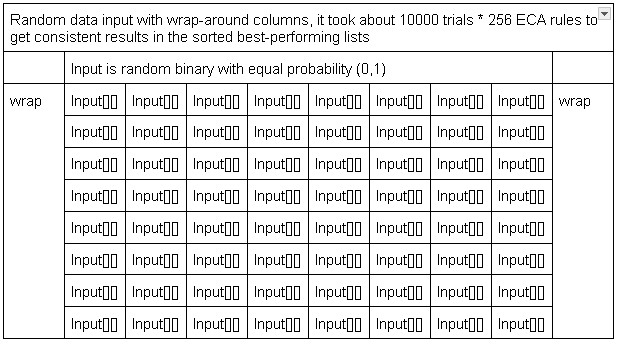
\includegraphics{WrappedInput}\\
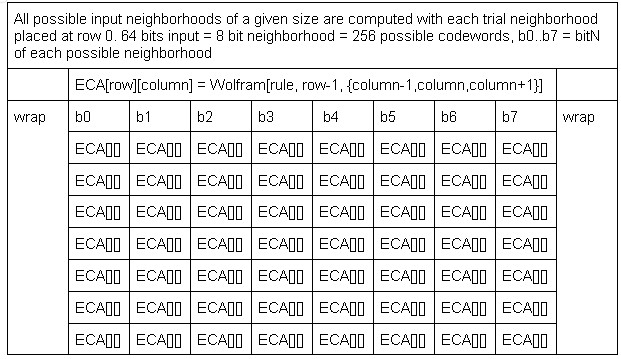
\includegraphics{ECAspace}\\
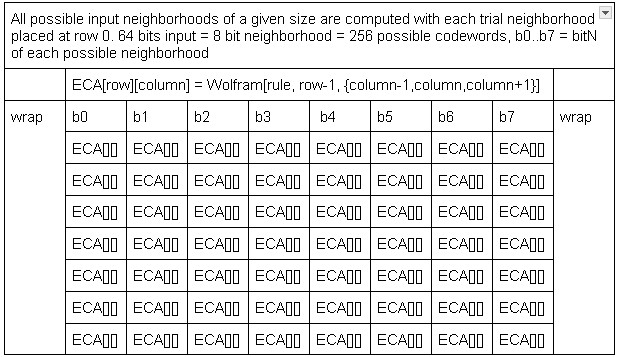
\includegraphics{ErrorScore}\\
Include graphics for: Input example, Codeword output example, Error map example

Various shapes and sizes of arrays


CDT of spectral method of solving DEs

voting() subfunction to increase accuracy

\bibliographystyle{plain}
\bibliography{HashBib.bib}

\end{document}